
\section{Introduction}


Modern machine learning (ML) workloads increasingly rely on GPUs, yet developing high-performance GPU programs remains challenging, especially for end-to-end workloads where performance depends on both GPU kernel efficiency and host-side settings (e.g., memory allocation and CPU–GPU overlap). 

While LLM-based code generation offers a promising path to automate GPU programming, existing methods—including multi-agent systems~\cite{cudaforge,cupilot,astra} and domain-specific fine-tuning or RL~\cite{kevin,cudal2}—focus on single-kernel optimization, limiting them to Level 1/2 tasks in KernelBench~\cite{kernelbench} (e.g., a 3D max-pooling kernel).



However, the central challenge lies in moving beyond kernel-level generation to full end-to-end GPU programs, which these methods do not support. In contrast, KernelBench~\cite{kernelbench} Level 3/4 workloads involve multiple interacting kernels and impose fundamentally different system-level requirements.
For example, the entire VisionTransformer model architecture~\cite{vit} in level 3,  whose end-to-end performance is dominated by factors that go beyond any single kernel: kernel fusion's boundaries, launch config, CPU–GPU synchronization, and data movement, which has been proven critical for GPU program performance~\cite{emogi,mobius,native,liberator}.



\begin{figure}[t]
    \centering
    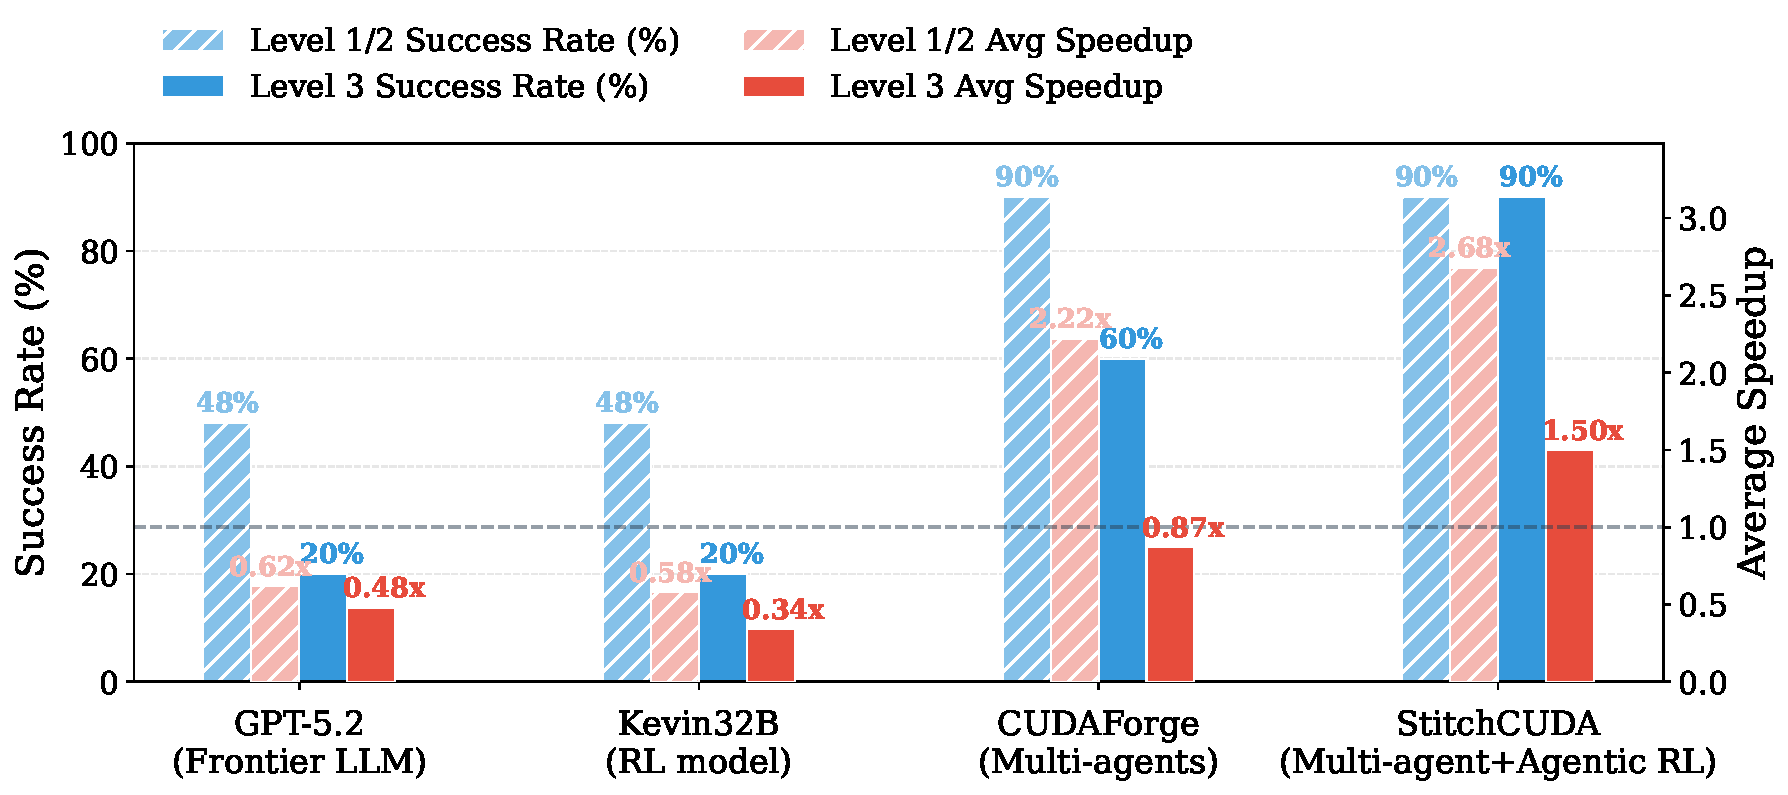
\includegraphics[width=\linewidth]{pic/level_comparison.pdf}
    \caption{The performance of various automated GPU program generation methods on KernelBench Level 1/2/3. Achieved average speedup is relative to PyTorch eager mode code, using NVIDIA H200 GPU.}
    \label{fig:l3}
    \vspace{-18pt}
\end{figure}



Recent multi-agent approaches such as CUDAForge and QiMeng~\cite{cudaforge,qimeng} leverage fine-grained prompt engineering and task decomposition (e.g., Coder and Verifier agents), showing promise on single kernels. However, they lack mechanisms for enforcing cross-kernel optimization and host-side orchestration. As shown in Fig.~\ref{fig:l3}, CUDAForge achieves near-perfect correctness with strong speedups on KernelBench Level 1/2, but struggles on Level 3 with lower success rates and performance gains.


In addition, according to our observation discussed in Section~\ref{sec:discuss}, the Coder's ability also limits the overall performance of current methods. 
A common approach to improve model
ability in a specific domain is Reinforcement Learning (RL), especially when rewards are verifiable
(a.k.a RLVR). Prior work~\cite{kevin,cudal2,li2025cudal1improvingcudaoptimization}
uses functional correctness and speedup over reference implementations as
verifiable rewards to train LLMs with GRPO, yielding measurable gains. However,
these rule-based rewards are vulnerable to \emph{reward hacking}, leading to undesirable behaviors such as writing PyTorch-only code or hardcoding the output without implementing a real program (see Appendix~\ref{app:rewardhack} for examples). Moreover, they
can induce degenerate solutions (e.g., only replacing a trivial operator such as a standalone \texttt{ReLU} in a Neural Network) that obtain nontrivial
reward yet do not correspond to meaningful improvements in kernel quality. Thus, an RL-trained model could achieve a high success rate, but fails to deliver effective optimization, as Kevin-32B shown in Fig.\ref{fig:l3}. 

More fundamentally, existing RLVR formulations mainly focus on kernel generation alone, without learning to incorporate \emph{structured} feedback (e.g., compiler diagnostics and profiling bottlenecks) to 
optimize code accordingly. As a result, the model often fails to reliably follow concrete feedback and implement targeted optimizations in an agentic framework, which directly undermines end-to-end optimization performance.
Agentic RL is a promising alternative because it directly trains the model to
operate within an agentic framework, where the model interacts with the environment, gets feedback, and conducts the next action. However, collecting multi-turn rollouts incurs
substantial computational overhead, making training very inefficient.





We summarized the following challenges according to our experiments and observations:

    \noindent \textbf{(C1) End-to-end program requires global coordination.}
    Unlike single-kernel optimization, end-to-end GPU program performance is dominated by intra-kernel decisions (e.g., kernel fusion boundaries, and memory footprint among kernels) and host-side orchestration; the automated generation needs to reason over a \emph{program-level} state rather than dealing with each kernel design individually. This complex end-to-end system design cannot be well addressed by one-shot LLM inference or a simple self-refine loop.
.
    
    \noindent \textbf{(C2) Coder's CUDA-specific coding capability needs to be improved beyond prompting.} %under real feedback from the execution environment.}
    Multi-agent decomposition can surface feedback from other agents to guide Coder, but without parameter updates, the Coder often cannot reliably execute nontrivial CUDA transformations (e.g., deriving a correct tiling strategy from profiling hints), thereby becoming the primary bottleneck in practice.


    \noindent \textbf{(C3) Direct RLVR fails to improve Coder's capability in end-to-end setting.} 
    Existing RLVR approaches for CUDA code generation are vulnerable to reward hacking and can induce degenerate solutions. More fundamentally, coders are not explicitly trained to interpret \emph{structured} execution feedback and to apply targeted improvements. While agentic RL could in principle address this gap, multi-turn rollouts are, however, prohibitively costly in realistic CUDA environments, making training extremely inefficient.

  
To apply LLMs in automated end-to-end GPU program generation and optimization, we propose StitchCUDA, a multi-agent framework integrated with rubric-based agentic reinforcement learning. StitchCUDA instantiates three specialized agents: a \textit{Planner} that decomposes the required task in reference PyTorch code into a program specification (kernel fusion boundaries, tensor shapes/layout contracts, and CPU-GPU overlapping), a \textit{Coder} that implements the host code and GPU kernels accordingly, and a \textit{Verifier} that enforces correctness checks and do the performance analysis using Nsight Systems (Nsys) and Nsight Compute (NCU), enabling an iterative “plan–code–profile–refine” loop for end-to-end GPU programming. 

Beyond multi-agent orchestration, we further improve the \textit{Coder} via rubric-based agentic reinforcement learning, enabling end-to-end optimization on a sequence of code-generation and optimization actions. To alleviate rollout overhead, we decompose multi-turn agentic RL into two \emph{atomic skills}: \textbf{(1) from-scratch generation}, translating high-level GPU programming tasks and reference code into a correct CUDA implementation; and \textbf{(2) feedback-driven optimization}, incorporating structured execution feedback (e.g., compiler diagnostics and profiling bottlenecks) to fix bugs and improve performance. We collect single-turn training data for both skills during workflow execution to train \textit{Coder}, which is substantially more efficient than multi-turn agentic RL.
Further, to address reward hacking and degenerate behaviors,
we combine rule-based rewards from real executions (functional correctness/measured end-to-end speedup) with expert-aligned rubric rewards produced by an advanced LLM (details in Section~\ref{RLdesign}), avoiding reward hacking and encouraging end-to-end system optimization.



Our key contributions are summarized below:
\begin{itemize}

\vspace{-0.2cm}
    \item We propose StitchCUDA, a multi-agent system that generates complete end-to-end GPU programs from task requirements and PyTorch references, integrated with an agentic RL technique to effectively improve the Coder's capability in this domain. We decompose end-to-end GPU programming tasks into three agents. We also prepare expert-level chains of thoughts (CoT) in prompt engineering and effective expertise tools for them, to better guide the Coder to address end-to-end program bottlenecks.   

    \vspace{-0.2cm}
    \item We decompose multi-turn agentic RL into atomic skills, substantially reducing rollout overhead while better aligning with the end-to-end task. Combined with fine-grained rubric rewards, our approach mitigates reward hacking/degenerate behavior and performs better.

    \vspace{-0.2cm}
    \item Comprehensive experiment results show that StitchCUDA performs outstandingly in the end-to-end GPU programming task. In our test sets derived from KernelBench Level 3, StitchCUDA achieves nearly 100\% success rate, and 1.5$\times$ average speedup than PyTorch eager (1.72$\times$$\uparrow$ than multi-agent approach, and 2.73$\times$$\uparrow$ than RL model).  
\end{itemize}
Code of the \textsc{StitchCUDA} framework is avalaible at https://github.com/UMN-APEX-Lab/StitchCUDA.

